% This is LLNCS.DEM the demonstration file of
% the LaTeX macro package from Springer-Verlag
% for Lecture Notes in Computer Science,
% version 2.4 for LaTeX2e as of 16. April 2010
%
\documentclass{llncs}

% allows for temporary adjustment of side margins
\usepackage{chngpage}

% just makes the table prettier (see \toprule, \bottomrule, etc. commands below)
\usepackage{booktabs}

\usepackage[utf8]{inputenc}

% URL handling
\usepackage{url}
\urlstyle{same}

% Todos
%\usepackage[colorinlistoftodos]{todonotes}
%\newcommand{\ke}[1]{\todo[size=\small, color=orange!40]{\textbf{Kai:} #1}}
%\newcommand{\tb}[1]{\todo[size=\small, color=green!40]{\textbf{Thomas:} #1}}


%\usepackage{makeidx}  % allows for indexgeneration

%\usepackage{amsmath}
\usepackage{amsmath, amssymb}
\usepackage{mathabx}

% monospace within text
\newcommand{\ms}[1]{\texttt{#1}}

% examples
\usepackage{fancyvrb}
\DefineVerbatimEnvironment{ex}{Verbatim}{numbers=left,numbersep=2mm,frame=single,fontsize=\scriptsize}

\newenvironment{gcotable-1}{
  \scriptsize
  \sffamily
  \vspace{0.3cm}
  \begin{tabular}{l|l|l|l|l|l}
  \hline
  \textbf{c. type} & \textbf{context concept} & \textbf{p. list} & \textbf{concepts} & \textbf{c. element} & \textbf{c. value} \\
  \hline

}{
  \hline
  \end{tabular}
  \linebreak
}

\newenvironment{gcotable}{
  \scriptsize
  \sffamily
  \vspace{0.3cm}
  \begin{tabular}{l|l|l|l|l|l|l}
  \hline
  \textbf{c. type} & \textbf{context concept} & \textbf{left p. list} & \textbf{right p. list} & \textbf{concepts} & \textbf{c. element} & \textbf{c. value} \\
  \hline

}{
  \hline
  \end{tabular}
  \linebreak
}

\newenvironment{DL}{
  %\scriptsize
  %\sffamily
  %\vspace{0.3cm}
	\begin{center}
  \begin{tabular}{r l}

}{
  \end{tabular}
	\end{center}
}

\usepackage{xspace}
% Einfache und doppelte Anfuehrungszeichen
\newcommand{\qs}{``} 
\newcommand{\qe}{''\xspace} 
\newcommand{\sqs}{`} 
\newcommand{\sqe}{'\xspace} 

% checkmark
\usepackage{tikz}
\def\checkmark{\tikz\fill[scale=0.4](0,.35) -- (.25,0) -- (1,.7) -- (.25,.15) -- cycle;} 

% Xs
\usepackage{pifont}

% Tabellenabstände kleiner
\setlength{\intextsep}{10pt} % Vertical space above & below [h] floats
\setlength{\textfloatsep}{10pt} % Vertical space below (above) [t] ([b]) floats
% \setlength{\abovecaptionskip}{0pt}
% \setlength{\belowcaptionskip}{0pt}

\usepackage{tabularx}
\newcommand{\hr}{\hline\noalign{\smallskip}} % für die horizontalen linien in tabellen

% pipe
%\usepackage[T1]{fontenc}

% Todos
\usepackage[colorinlistoftodos]{todonotes}
\newcommand{\ke}[1]{\todo[size=\small, color=orange!40]{\textbf{Kai:} #1}}
\newcommand{\tb}[1]{\todo[size=\small, color=green!40]{\textbf{Thomas:} #1}}

\setcounter{secnumdepth}{5}

\begin{document}

%
%
\title{XXXXX}
%
\titlerunning{XXXXX}  % abbreviated title (for running head)
%                                     also used for the TOC unless
%                                     \toctitle is used
%
\author{XXXXX\inst{1} \and XXXXX\inst{2}}
%
\authorrunning{XXXXX} % abbreviated author list (for running head)
%
%%%% list of authors for the TOC (use if author list has to be modified)
\institute{XXXXX\\
\email{XXXXX},\\ 
\and
XXXXX \\
\email{XXXXX} 
}

\maketitle              % typeset the title of the contribution

\begin{abstract}


\keywords{..}
\end{abstract}
%

% ---------------

\section{Introduction}

\section{Notes}

\begin{itemize}
	\item requirements / constraints mapped to DL
	\item requirements / constraints which cannot be mapped to DL
	\item syntactic sugar for some constraints
	\item complex constraints encompass complex constraints and simple constraints
	\item DL statements of complex constraints are created out of DL statements of composed constraints 
	\item define terminology for RDF constraints
\end{itemize}

\section{Motivation}

At-least restrictions can be expressed either generically by description logics (DL) or specifically by domain-specific constraint languages (DSCL) such as OWL 2, DSP, and ShEx.
With at-least restrictions we can state that having at least 2 female childs is equivalent to having at least 2 daughters. This axiom may be represented by DL in a logical way:

\begin{align*}
Having2Daughters \equiv \geq 2 hasChild.Woman
\end{align*}

The same axiom may also be represented by different DSCLs like OWL 2, DSP, and ShEx:

\begin{ex}
# OWL 2
# -----
:Having2Daughters
    a owl:Restriction ;
    owl:minQualifiedCardinality "2"^^xsd:nonNegativeInteger ;
    owl:onProperty :hasChild ;
    owl:onClass :Woman .
		
# DSP
# ---			
:descriptionTemplate 
    a dsp:DescriptionTemplate ; 
    dsp:resourceClass :Having2Daughters ; 
    dsp:statementTemplate [
        a dsp:NonLiteralStatementTemplate ;
        dsp:minOccur "1"^^xsd:nonNegativeInteger ; 
        dsp:maxOccur "infinity"^^xsd:string ; 
        dsp:property :hasChild ; 
        dsp:nonLiteralConstraint [ 
            a dsp:NonLiteralConstraint ;
            dsp:valueClass :Woman ] ] .

# ShEx
# ----
<Having2Daughters> {         
    :hasChild @<Woman>{2, }
}
<Woman> {         
    rdf:type (:Woman)
}
\end{ex}

Data, which is valid according to the specified at-least restriction, looks like this:

\begin{ex}
:Marge
    a :Having2Daughters , :Woman ;
    :hasChild :Maggie , :Lisa .
:Maggie
    a :Woman .
:Lisa
    a :Woman .
\end{ex}

If :Marge has only 1 child and if :Marge is assigned to the class :Having2Daughters, a constraint violation is raised for the following invalid data:

\begin{ex}
:Marge
    a :Having2Daughters , :Woman ;
    :hasChild :Lisa .
:Lisa
    a :Woman .
\end{ex}

As there is no standard constraint language, constraint designers may choose different DSCLs in order to express the same at-least restriction. 
When constraint designers choose one DSCL in order to express an arbitrary constraint, it should be possible to transform this constraint into a constraint expressed by any other DSCL. 
This is important as it is often the case that one constraint designer knows to read and to write constraints in one DSCL very well but not in another DSCL. 
This way, constraint designers may communicate with each other without the necessity to understand the other DSCL.

There are validation environments available enabling to automatically validate any RDF constraints expressed by just a few DSCL such as OWL 2 and DSP.
But it should be possible to validate any RDF constraints expressed by any DSCL automatically and what is even more important in the same manner without any differences.  

The following table contains the mapping between the at-least restriction expressed by description logics and the at-least restriction expressed by a generic constraint language conforming to an ontology describing constraint languages.
Each constraint is either a constraint on classes or a constraint on properties.

\begin{gcotable}
property & Having2Daughters & hasChild & - & Woman & $\geq$ & 2 \\
\end{gcotable}


The at-least restriction (expressed by the generic constraint language) is represented in RDF as follows:

\begin{ex}
:minCardinalityConstraint
    a gclo:PropertyConstraint ;
    gclo:contextConcept :Having2Daughters ;
    gclo:propertyList ( :hasChild ) ;
    gclo:concept :Woman ;
    gclo:constrainingElement "\geq" ;
    gclo:constrainingValue "2" .
\end{ex}

We implement an automatic validation for any constraint expressed by a generic constraint language conforming to an ontology describing constraint languages.
If we transform a specific constraint (expressed by any DSCL) into a generic constraint (expressed by the generic constraint language), we will be able to validate the generic constraint and therefore the specific constraint immediately. 
As a consequence, we do not have to specify an automatic validation for each specific constraint, as we need to define an automatic validation once for each generic constraint. The underlying SPARQL query is executed within the SPIN validation environment:

\begin{ex}
# constraint
# ----------
?propertyConstraint
    a gclo:PropertyConstraint ;
    gclo:contextConcept ?contextConcept ;
    gclo:propertyList ( ?property ) ;
    gclo:concept ?concept ;
    gclo:constrainingElement ?constrainingElement ;
    gclo:constrainingValue ?constrainingValue .
		
# data
# ----
?this ?property ?o .
?this rdf:type ?contextConcept .

# validation ( at-least restriction )
# -----
FILTER ( ?constrainingElement = "\geq" ) .
BIND ( owl2spin:qualifiedCardinality( ?this, ?property, ?concept ) AS ?c ) .
BIND( STRDT ( STR ( ?constrainingValue ), xsd:nonNegativeInteger ) AS ?MinimumCardinality )
BIND( STRDT ( STR ( ?c ), xsd:nonNegativeInteger ) AS ?cardinality )
FILTER ( ?cardinality < ?MinimumCardinality ) .		  
\end{ex}

When domain experts use graphical user interfaces to define constraints in a user-friendly way, 
these constraints can be either mapped to either a specific or a generic constraint, as for both an automatic validation is provided in the background.    
So, the user does not have to know how to express specific constraints using a DSCL such as OWL 2, DSP, or ShEx.
If there is a new constraint not covered by any DSCL you can just define the automatic validation for this newly defined constraint.
This way, you are able to extend existing DSCL and to define new DSCL if existing DSCLs are not sufficient for further use cases.

Our \textbf{contributions} of this paper are:
\begin{enumerate}
	\item each constraint (expressed by any DSCL) can be validated automatically
	\item any specific constraint (expressed by any DSCL) can be transformed into a generic constraint (expressed by a generic constraint language)
	\item we developed an ontology describing any constraint language
\end{enumerate}

Benefits:
\begin{itemize}
	\item GCL with only 6 elements
	\item if a language designer develops a new DSCL the language designer only needs to define a mapping between the new DSCL and the GCLO 
	in order to be able to automatically validate the new DSCL constraints
\end{itemize}

\section{Ideas}

idea:
\begin{itemize}
	\item each specific constraint expressed using any domain specific language can be expressed as DL constraint using DL
	\item each DL constraint can be expressed as generic constraint using generic constraint language
	\item meta-model based ontology describing constraints
	\item possible limitation: maybe only typical constraints
\end{itemize}

purpose:
\begin{itemize}
	\item translations of constraints expressed using any domain specific constraint language
\end{itemize}

contributions:
\begin{itemize}
	\item 
\end{itemize}

assumption:
\begin{itemize}
	\item CWA
\end{itemize}


ontology design pattern.org
constraint grammar
constraint elements are the same
DSP uses other design pattern / 
constraint / constraint elements / constraint design patterns / constraint language
define terminology
related to requirements DB / relate requirements to constraints, constraint languages
constraint element: e.g. min cardinality
dependency between requirements / when this requirements is fulfilled then this is also fulfilled (e.g. min card and requ. car)
min car more powerful than req. propery
why ontology? automatic translation from DSP to OWL 
define general constraint language
we do not invent a new constraint languages
requirements in SPARQL umsetzten
only one validation for each requirement
constraints may be composed 

\begin{itemize}
	\item any specific constraint (expressed by DSCL) must be mapped to a generic constraint (expressed by GCL)
\end{itemize}

\section{An Ontology Describing Constraint Languages} 

fig:generic constraint language ontology.  
\begin{figure}
	\centering
		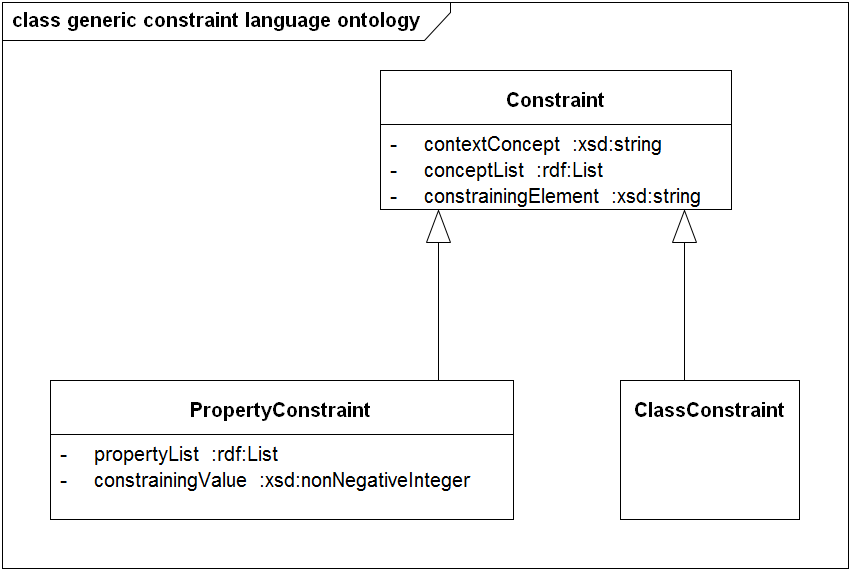
\includegraphics[width=1.00\textwidth]{generic constraint language ontology/generic constraint language ontology.png}
	\caption{generic constraint language ontology}
	\label{fig:generic constraint language ontology}
\end{figure}

terminology:
\begin{itemize}
	\item A "constraint" is an actual constraint, like dcterms:creator :hasMinCardinality "1" .
  \item a "constraint language" like DSP is used to formulate constraints.
  \item a constraint language consists of "constraint elements" like :hasMinCardinality (this is probably the most controverse definition).
	\item class constraint: constraint on context class
\end{itemize}

\begin{itemize}
	\item relationship to requirement
  \item ontology describing constraint languages
	\item interoperability between constraint languages
  \item express constraint in CL A and translate constraint in CL B
  \item provide SPARQL validation (SPIN mapping) for each general C 
\end{itemize}

\section{Complex Constraints}

\subsection{Disjoint Classes}

\begin{DL}
Hologram $\sqcap$ Human $\sqsubseteq$ $\perp$\\
Alternative:\\
$Hologram \sqsubseteq \neg Human$
\end{DL}

\subsection{Minimum Qualified Cardinality Restrictions on Properties}

\begin{DL}
$FederationCaptain \sqsubseteq Federation \sqcap \geq1 commandsVessel . Vessel $
\end{DL}

\section{Syntactic Sugar}

In Section 1.3 we introduced three forms of RBox axioms: role inclusions, role equiv-
alences and role disjointness. OWL provides a variety of others, namely role transi-
tivity, symmetry, asymmetry, reflexivity and irreflexivity. These are sometimes consid-
ered as basic axiom types in DLs as well, using some suggestive notation such as
Trans( ancestorOf ) to express that the role ancestorOf is transitive. However, such axioms
are just syntactic sugar; all role characteristics can be expressed using the features
of DLs that we have already introduced.

\begin{itemize}
  \item domain and range
	\item (ir)reflexive object properties
	\item Exact Qualified Cardinality Restrictions on Properties
\end{itemize}

\bibliography{../../literature/literature}{}
\bibliographystyle{plain}
\setcounter{tocdepth}{1}
%\listoftodos
\end{document}
